\documentclass[11pt]{article}

% ---------------------------------------------------------------------------
% Beacon: Direct Multi-Horizon Gradient Boosting with Target-Hour Weather
% Forecasts for Day-Ahead Zonal Load Forecasting in ISO New England
%
% Build:  pdflatex main && bibtex main && pdflatex main && pdflatex main
% (or upload the paper/ folder to Overleaf)
% ---------------------------------------------------------------------------

\usepackage[T1]{fontenc}
\usepackage{lmodern}
\usepackage[margin=1in]{geometry}
\usepackage{graphicx}
\usepackage{booktabs}
\usepackage{amsmath,amssymb}
\usepackage{siunitx}
\usepackage{microtype}
\usepackage[hidelinks]{hyperref}
\usepackage{caption}
\usepackage{xcolor}

\graphicspath{{figures/}}
\captionsetup{font=small,labelfont=bf}

\title{\textbf{Beacon: Direct Multi-Horizon Gradient Boosting with\\
Target-Hour Weather Forecasts for Day-Ahead Zonal Load\\
Forecasting in ISO New England}}

\author{Arun Surendranath\\[2pt]
\small Independent Researcher\\
\small \href{https://github.com/arunnath011/NEMA}{github.com/arunnath011/NEMA}}

\date{\today}

\begin{document}
\maketitle

\begin{abstract}
Day-ahead electricity load forecasting underpins unit commitment, economic
dispatch, and reserve sizing in wholesale power markets, where small accuracy
gains yield large cost and reliability benefits. We study 24-hour-ahead hourly
load forecasting for the NEMA (Northeast Massachusetts/Boston) zone of ISO New
England and present \emph{Beacon}, a direct multi-horizon gradient-boosting
forecaster comprising 24 CatBoost models---one per horizon $h=1,\dots,24$---each
predicting its step directly from a 168-hour lookback window, thereby avoiding
recursive error compounding. Each horizon model is conditioned on
\emph{target-hour} exogenous features: the exactly-known calendar and the
\emph{forecasted} weather at the target hour $t{+}h$, the dominant driver of
day-ahead load. We further unify the training and serving weather source on
Open-Meteo (ERA5 archive for history, forecast API for deployment), removing a
train/serve distribution mismatch that otherwise nearly doubled day-ahead error.
On a strictly held-out 2025 test set, Beacon attains a day-ahead ($h{=}24$) MAE
of 76.7~MW and an $h{=}1$ $R^2$ of 0.977. In a horizon-matched live evaluation
over 30 days, Beacon achieves a day-ahead MAE of 89.3~MW, slightly improving on
ISO New England's operational day-ahead forecast (92.6~MW). A shuffled-target
audit confirms the model exploits genuine feature--target structure rather than
leakage. The pipeline is keyless and fully reproducible.

\end{abstract}

\smallskip
\noindent\textbf{\small Keywords:}~{\small short-term load forecasting; day-ahead
forecasting; multi-horizon forecasting; gradient boosting; CatBoost;
weather-informed forecasting; ISO New England.}
\medskip

\section{Introduction}\label{sec:intro}

Short-term electricity load forecasting is a foundational input to the operation
of wholesale power markets. Independent system operators rely on accurate
day-ahead demand forecasts to schedule generation through unit commitment, to
clear economic dispatch, and to size operating reserves. Because these decisions
trade off the cost of committed capacity against the risk of shortfall, even
modest reductions in forecast error translate into appreciable savings and
improved reliability across a control area. The day-ahead horizon is
particularly consequential: commitment decisions for slow-starting units are
made roughly a day in advance, so accuracy 24~hours out directly shapes the cost
and security of the resulting schedule.

We study this problem for the NEMA zone (Northeast Massachusetts/Boston) of ISO
New England, identified as load zone \texttt{.Z.NEMASSBOST} (location id 4008).
A natural and demanding reference point is the operator's own product: ISO New
England publishes an operational day-ahead reliability-region demand forecast
that market participants and operators rely upon \cite{isone}. Improving on this
forecast is a meaningful and hard bar, precisely because it is the number the
system already trusts. Our goal is therefore not merely to fit historical load
well, but to match or exceed the operational benchmark on a like-for-like basis.

In pursuing that goal we highlight and correct two methodological pitfalls that
recur in applied load-forecasting work. The first is \emph{horizon mismatch}:
comparing a model's short-lead nowcast (e.g.\ a 1-hour-ahead prediction) against
an operator's day-ahead forecast, which flatters the model by pitting an easier
task against a harder one. We instead evaluate both forecasters at the same
24-hour-ahead horizon. The second is a \emph{train/serve weather-source
mismatch}: training on weather from one provider while serving live predictions
with weather from another silently degrades deployed accuracy, because the model
learns the idiosyncrasies of the training source. We find this single mismatch
nearly doubles live day-ahead error, and that unifying the source on Open-Meteo
\cite{openmeteo} removes most of the gap to the operator.

Methodologically, we adopt a \emph{direct multi-horizon} design. Rather than
training one model and recursively rolling its predictions forward---which
compounds errors and, for load, forces a single-phase predictor to serve the
opposite phase of the diurnal cycle---we train 24 independent CatBoost
\cite{prokhorenkova2018catboost} models, one per horizon $h=1,\dots,24$, each
predicting directly from a 168-hour (one-week) lookback window. Crucially, each
horizon model receives \emph{target-hour} exogenous features: the calendar
encoding at $t{+}h$, which is known exactly, together with the forecasted
weather at $t{+}h$, the dominant driver of load a day ahead.

\paragraph{Contributions.} This paper makes the following contributions.
\begin{itemize}
  \item A direct per-horizon forecaster (\emph{Beacon}) of 24 CatBoost models
        that removes recursive error compounding, achieving on average 80.6\%
        lower MAE across the 24-hour horizon than a single-model roll-out.
  \item Target-hour exogenous features (exact calendar plus forecast weather at
        $t{+}h$) as the principal lever for day-ahead accuracy, cutting
        held-out day-ahead MAE from 183 to 77~MW.
  \item Identification and correction of a train/serve weather-source mismatch,
        which reduces live day-ahead MAE from roughly 147 to 90~MW---a
        deployment lesson rarely reported in the literature.
  \item A horizon-matched evaluation protocol against ISO New England's
        operational day-ahead forecast, paired with a rigorous leakage audit via
        a shuffled-target test.
  \item A fully reproducible, keyless, and deployable pipeline built on ISO-NE
        Web Services and Open-Meteo.
\end{itemize}

On a strictly held-out 2025 test set Beacon attains a day-ahead MAE of 76.7~MW
and an $h{=}1$ $R^2$ of 0.977, and in a horizon-matched 30-day live evaluation
it reaches a day-ahead MAE of 89.3~MW against ISO New England's 92.6~MW.

The remainder of the paper is organized as follows.
Section~\ref{sec:related} situates the work within the load-forecasting
literature. Section~\ref{sec:data} describes the load, weather, and benchmark
data. Section~\ref{sec:method} details the feature construction and the direct
multi-horizon model, and Section~\ref{sec:setup} specifies the evaluation
protocol. Section~\ref{sec:results} reports the results, Section~\ref{sec:discussion}
discusses the findings, and Sections~\ref{sec:limits} and~\ref{sec:conclusion}
cover limitations and conclusions.

\section{Related Work}\label{sec:related}

\paragraph{Statistical methods.} Classical short-term load forecasting has long
relied on linear time-series models. Autoregressive integrated moving-average
(ARIMA) models and exponential-smoothing (ETS) methods remain standard baselines
for seasonal demand series \cite{box2015time,hyndman2018forecasting}. These
methods are interpretable and data-efficient, but they capture exogenous drivers
such as weather only through limited regression terms and struggle with the
strongly nonlinear, multi-seasonal structure of hourly electricity load.

\paragraph{Gradient-boosted trees.} Tree-based gradient boosting has become a
dominant approach for tabular forecasting, combining strong accuracy with modest
tuning effort. XGBoost \cite{chen2016xgboost} and LightGBM \cite{ke2017lightgbm}
popularized scalable boosting, while CatBoost \cite{prokhorenkova2018catboost}
adds ordered boosting and native categorical handling that suit the calendar-
and weather-derived features common in load forecasting. Such models naturally
ingest engineered lag, calendar, and degree-day features and handle nonlinear
interactions without bespoke architectures, which motivates our choice of
CatBoost as the per-horizon learner.

\paragraph{Deep learning.} Neural sequence models offer an alternative for
temporal demand. Long short-term memory networks \cite{hochreiter1997lstm}
capture long-range dependencies, and transformer-based forecasters extend this
to long sequences: the Informer \cite{zhou2021informer} reduces the quadratic
cost of attention for long-horizon prediction, and the Temporal Fusion
Transformer \cite{lim2021temporal} integrates static and time-varying exogenous
covariates with interpretable attention. These models can be powerful but are
data-hungry and comparatively costly to train, deploy, and reproduce in an
operational, single-zone setting.

\paragraph{Multi-horizon strategies.} Producing a full 24-hour profile requires
a strategy for mapping inputs to multiple lead times. The principal options are
\emph{recursive} roll-out, which feeds predictions back as inputs and thereby
compounds errors and propagates bias, and \emph{direct} forecasting, which
trains a separate model per horizon \cite{taieb2016bias}. The recursive--direct
trade-off has been studied extensively, with direct strategies favored when bias
accumulation dominates. We adopt the direct strategy and, as shown later,
observe that a single-model roll-out degrades catastrophically at mid-horizons
because a short-lead predictor is forced onto the opposite phase of the diurnal
cycle.

\paragraph{Weather-informed and probabilistic load forecasting.} Weather is the
dominant exogenous driver of load, and the broader literature on probabilistic
and weather-informed electric load forecasting establishes both the centrality
of temperature-derived features and the value of honest, well-specified
evaluation \cite{hong2016probabilistic}. Degree-day and thermal-stress
transforms are standard levers for encoding the nonlinear load--temperature
response.

\paragraph{Gap.} Across these strands, two practical issues remain
under-addressed. First, model-versus-operator comparisons are frequently made at
mismatched horizons, overstating gains. Second, the gap between a model's
back-tested accuracy and its deployed accuracy---driven here by a train/serve
weather-source mismatch---is rarely measured or reported. This work fills that
gap by combining a direct multi-horizon CatBoost forecaster with target-hour
forecast-weather features, unifying the train and serve weather source, and
evaluating against an operational ISO forecast on a strictly horizon-matched
basis with an explicit leakage audit.

\section{Data}\label{sec:data}

This study targets the Northeast Massachusetts / Boston (NEMA) load zone of
ISO New England (ISO-NE), identified as load zone \texttt{.Z.NEMASSBOST} and
ISO-NE location id 4008. Three data sources are combined: historical and live
zonal load, weather observations and forecasts, and an operational day-ahead
demand benchmark.

\subsection{Load data}

The training target is the ISO-NE hourly wholesale-load series (RTLO) for NEMA,
covering 2017-03-01 through 2025-11-30, comprising 76{,}719 hourly observations
after cleaning. For live serving, load is drawn from the ISO-NE Web Services API
endpoint \texttt{realtimehourlydemand} (location 4008), which publishes with a
settlement lag of approximately four days; hourly demand from the U.S. Energy
Information Administration (EIA) is used as a fallback when ISO-NE data are
unavailable~\cite{eia930}. The two series differ slightly, as the
wholesale-load (WHLSECOST) history and the real-time demand series are not
identical products.

\subsection{Weather data}

Weather is obtained from Open-Meteo~\cite{openmeteo} for the Boston Logan station
(42.3656$^{\circ}$\,N, $-71.0096^{\circ}$\,W). The variables used are
temperature, relative humidity, wind speed, dew point, cloud cover, apparent
temperature, and visibility (in $^{\circ}$F, mph, and \%). Critically, a single
provider supplies both training history and live serving: the Open-Meteo archive
API (backed by ERA5 reanalysis) furnishes the historical record, while the
Open-Meteo forecast API supplies weather at serving time. Neither requires an API
key. This deliberate train/serve source unification removes a distribution
mismatch that otherwise degrades deployed day-ahead accuracy. The Open-Meteo
archive omits visibility, which is filled with a constant.

\subsection{Benchmark}

As an operational baseline we use ISO-NE's official day-ahead demand forecast for
NEMA, retrieved from the ISO-NE Web Services \texttt{dayaheadhourlydemand}
endpoint (location 4008)~\cite{isone}. This is the forecast that ISO-NE operators
rely on for unit commitment and reserve planning, and constitutes a meaningful,
hard bar for any candidate model.

\subsection{Temporal split, cleaning, and imputation}

To prevent any leakage of future information into model fitting, the data are
divided by a strict temporal split at \texttt{TRAIN\_CUTOFF}
$=$ 2024-12-31 23:00. All observations at or before the cutoff form the training
partition (68{,}704 rows) and all later observations form the held-out test
partition (8{,}015 rows). Because the model consumes fixed-length lookback
windows (Section~\ref{sec:method}), sequence construction yields 58{,}236
training, 10{,}276 validation, and 7{,}823 test windows, where the validation
set is the most recent 15\% of the training partition. Table~\ref{tab:data}
summarizes the partition sizes.

Cleaning and imputation are performed using statistics estimated on the training
partition only: missing values are filled with train-only medians, so that no
test-period information influences the imputation of any feature. Combined with
the temporal split, this ensures that every fitting decision depends solely on
information available at or before the cutoff.

\begin{table}[t]
\centering
\caption{NEMA load data partitions under the strict temporal split at
2024-12-31 23:00.}
\label{tab:data}
\begin{tabular}{lrr}
\toprule
Partition & Rows & Windows \\
\midrule
Train      & 68{,}704 & 58{,}236 \\
Validation & --       & 10{,}276 \\
Test       & 8{,}015  & 7{,}823 \\
\midrule
Total      & 76{,}719 & --       \\
\bottomrule
\end{tabular}
\end{table}

\section{Methodology}\label{sec:method}

\subsection{Notation and problem setup}

Let $y_t$ denote the NEMA hourly load at time $t$. Forecasting is performed from a
fixed-length lookback window of $L = 168$ hours, i.e. the one-week interval
$[t-L,\, t-1]$. For each forecast origin $t$ and each horizon
$h \in \{1, \dots, 24\}$, the task is to predict the load $y_{t+h}$ at the target
hour $t+h$. We adopt a \emph{direct} multi-horizon strategy: a separate model is
trained for each horizon $h$, mapping a feature vector to a single scalar target
$y_{t+h}$, with no recursive feedback of intermediate predictions.

\subsection{Window lag features}

The first feature block summarizes the lookback window
$[t-L,\, t-1]$. From each engineered channel we extract values at lags
$\{1, 4, 8, 24, 48, 168\}$ hours and rolling means over windows of $\{24, 168\}$
hours, capturing recent dynamics together with daily and weekly periodicity. The
raw load channel (RTLO) is restricted to a whitelist retained from a notebook
ablation --- \texttt{RTLO\_lag4}, \texttt{RTLO\_mean24}, \texttt{RTLO\_lag48},
\texttt{RTLO\_lag168}, and \texttt{RTLO\_mean168} --- which avoids redundant
near-term load lags while preserving the daily and weekly
load signal. The full window feature map, denoted $\phi_{\mathrm{lag}}(\cdot)$,
produces 173 features.

\subsection{Calendar features}

Calendar effects are encoded with cyclic (sine/cosine) transforms of the hour of
day, day of week, and month, together with binary indicators \texttt{is\_weekend}
and \texttt{is\_us\_holiday}. The cyclic encoding avoids artificial discontinuities
at period boundaries (e.g. hour 23 to hour 0) and lets tree splits exploit smooth
diurnal, weekly, and seasonal structure.

\subsection{Weather-derived features}

Temperature drives electricity demand non-linearly through both heating and
cooling load. We compute heating and cooling degree days relative to a 65$^{\circ}$F
base,
\begin{equation}
\mathrm{HDD} = \max(0,\ 65 - T), \qquad
\mathrm{CDD} = \max(0,\ T - 65),
\end{equation}
together with the squared terms $T^2$, $\mathrm{HDD}^2$, and $\mathrm{CDD}^2$ to
capture curvature, and sigmoidal thermal-stress transforms (logistic functions
centred at 18$^{\circ}$C for heating and 22$^{\circ}$C for cooling) that model the
saturating onset of heating and air-conditioning demand. These derived quantities
are computed from the Open-Meteo weather variables described in
Section~\ref{sec:data}.

\subsection{Target-hour exogenous features}

The central methodological idea is to provide each horizon model with information
about the target hour $t+h$ itself, rather than only the history up to $t-1$. The
target-hour exogenous block $\phi_{\mathrm{exog}}(t+h)$ comprises all engineered
calendar features and all weather-derived features \emph{evaluated at the target
hour} $t+h$ --- the exactly-known calendar attributes of $t+h$ and the
\emph{forecasted} weather at $t+h$. The raw load channel RTLO is excluded from
this block, since the load at $t+h$ is precisely the prediction target. This block
contributes 21 features.

\subsection{Augmented feature map}

For each horizon $h$, the window features and the target-hour exogenous features
are concatenated into a single augmented vector:
\begin{equation}
\mathbf{x}_h \;=\; \bigl[\, \phi_{\mathrm{lag}}\!\bigl([t-L,\, t-1]\bigr)
\;;\; \phi_{\mathrm{exog}}(t+h) \,\bigr],
\label{eq:augmented}
\end{equation}
yielding a $173 + 21 = 194$-dimensional representation. Each horizon model
$f_h$ then predicts
\begin{equation}
\hat{y}_{t+h} \;=\; f_h(\mathbf{x}_h).
\end{equation}
The window block is shared in form across horizons, while the exogenous block
$\phi_{\mathrm{exog}}(t+h)$ shifts to the appropriate target hour for each $h$.

\subsection{Direct multi-horizon strategy}

We instantiate 24 independent CatBoost models, $\{f_h\}_{h=1}^{24}$, one per
horizon, each trained directly on its own target $y_{t+h}$. This contrasts with a
recursive roll-out, in which a single one-step model is applied iteratively, its
predictions fed back as inputs for subsequent steps. Recursive roll-out compounds
errors across steps and suffers from a train/serve mismatch, because at training
time the model conditions on true past values whereas at inference time it
conditions on its own noisy forecasts~\cite{taieb2016bias}. The direct strategy
trains each horizon under exactly the conditions it faces at deployment, removing
both error compounding and that mismatch, at the cost of fitting 24 models. For
ablation we also consider a single $h{=}1$ model whose prediction is reused for
every horizon.

\subsection{Learner and training configuration}

Each $f_h$ is a CatBoost gradient-boosted tree ensemble~\cite{prokhorenkova2018catboost},
chosen for strong tabular performance and native handling of the heterogeneous
engineered features. All 24 models share the same configuration: 1000 boosting
iterations, tree depth 8, learning rate 0.05, mean-absolute-error (MAE) loss,
early stopping after 50 rounds without validation improvement, and random seed 42.
The MAE objective aligns training directly with the primary evaluation metric and
is robust to occasional load spikes. Early stopping uses the validation split
defined in Section~\ref{sec:data}.

\subsection{Why target-hour weather is causal, not leakage}

A natural concern is whether conditioning on quantities at $t+h$ introduces
target leakage. It does not. The target-hour weather in $\phi_{\mathrm{exog}}(t+h)$
is a \emph{forecast}, which is exactly the quantity available to an operator at
prediction time; in deployment it is supplied by the Open-Meteo forecast API, and
in evaluation the corresponding archive value plays this role. The calendar
attributes of $t+h$ are deterministic and known arbitrarily far in advance.
Crucially, the load channel RTLO at $t+h$ --- the only quantity that would
constitute leakage --- is explicitly excluded from the exogenous block, and every
lag and rolling feature in $\phi_{\mathrm{lag}}$ references data at or before
$t-1$. No feature can therefore carry target-time load information, a property we
verify empirically with a shuffled-target audit in the results.

\section{Experimental Setup}\label{sec:setup}

\subsection{Temporal split and validation}
All evaluation respects the arrow of time. We impose a strict temporal split at
\texttt{TRAIN\_CUTOFF}~$=$~2024-12-31 23:00: every observation on or before the
cutoff is available for training, and the entire held-out test set lies in 2025.
At the raw-row level this yields $68{,}704$ training rows and $8{,}015$ test rows.
After constructing the $168$-hour lookback windows required by the model, the data
comprise $58{,}236$ training, $10{,}276$ validation, and $7{,}823$ test windows. The
validation set is the most recent $15\%$ of the training period and is used solely
for CatBoost early stopping (a $50$-round patience). No test-set information is used
at any point in feature construction, model selection, or hyper-parameter choice,
so the test set is a clean out-of-sample probe of generalisation to a future year.

\subsection{Metrics}
We report three standard regression metrics. Let $y_i$ denote the actual load,
$\hat{y}_i$ the forecast, $\bar{y}$ the mean of the actuals, and $N$ the number of
evaluated points. The mean absolute error (MAE, in MW),
\begin{equation}
\mathrm{MAE} = \frac{1}{N}\sum_{i=1}^{N}\bigl|\,y_i-\hat{y}_i\,\bigr|,
\end{equation}
is our primary metric because it shares the units of load and matches the model's
training loss. The mean absolute percentage error (MAPE, in \%),
\begin{equation}
\mathrm{MAPE} = \frac{100}{N}\sum_{i=1}^{N}\left|\frac{y_i-\hat{y}_i}{y_i}\right|,
\end{equation}
gives a scale-free view, and the coefficient of determination,
\begin{equation}
R^{2} = 1 - \frac{\sum_{i=1}^{N}\bigl(y_i-\hat{y}_i\bigr)^{2}}
                  {\sum_{i=1}^{N}\bigl(y_i-\bar{y}\bigr)^{2}},
\end{equation}
measures the fraction of load variance explained. On the held-out test set, metrics
are reported per horizon $h \in \{1,\dots,24\}$ and averaged across horizons.

\subsection{Baselines}
We compare Beacon against four references. (i) \emph{Persistence} carries the last
observed load forward. (ii) \emph{Seasonal-na\"ive} (168\,h) predicts the load
exactly one week earlier, exploiting the strong weekly periodicity of demand.
(iii) The \emph{single-model rolled-out} baseline trains a single $h=1$ model and
reuses its prediction for every horizon; this isolates the value of the direct
multi-horizon design and is the principal ablation contrast in
Section~\ref{sec:results}. (iv) The \emph{ISO-NE operational day-ahead forecast},
ISO New England's own published demand forecast for the NEMA reliability region
(location 4008), is the hardest and most operationally meaningful bar.

\subsection{Live, horizon-matched protocol}
A persistent pitfall in model-versus-operator comparisons is horizon mismatch:
contrasting a model's $1$-hour nowcast against a day-ahead operational benchmark.
We avoid this with a strictly horizon-matched live protocol. Over the most recent
$\sim$30-day window ($720$ hourly points), both forecasters are evaluated at the
\emph{same} $24$-hour-ahead horizon, both are driven by the \emph{same} Open-Meteo
weather, and both are scored against the same ground truth: ISO-NE
\texttt{realtimehourlydemand} actuals for location 4008. This like-for-like setup
is the basis for the live results in Table~\ref{tab:iso}. Because the live window
is short and falls in spring/early-summer, it complements rather than replaces the
larger held-out 2025 test set.

\subsection{Reproducibility}
All results are reproducible from the public repository
(\texttt{github.com/arunnath011/NEMA}). Running
\texttt{python -m nema\_forecast.model.train} regenerates the $24$ per-horizon
models and all metric artefacts (\texttt{model\_performance.json},
\texttt{horizon\_mae.json}); the data pipeline is keyless, drawing on ISO-NE Web
Services and Open-Meteo. The CatBoost configuration (1000 iterations, depth 8,
learning rate 0.05, MAE loss, seed 42) is fixed for every horizon model.

\section{Results}\label{sec:results}

We organise the evaluation around four questions. Section~\ref{sec:setup} first
establishes Beacon's accuracy on the held-out 2025 test set
(Table~\ref{tab:headline}, Figure~\ref{fig:horizon}); we then turn to the live,
horizon-matched comparison against ISO-NE's operational forecast
(Table~\ref{tab:iso}); isolate the contributions of the target-hour features and
the unified weather source (Table~\ref{tab:ablation}, Figure~\ref{fig:ablation});
and finally audit the pipeline for data leakage (Table~\ref{tab:leak}). Throughout,
test-set numbers refer to the $7{,}823$ held-out windows from 2025, whereas the
live numbers refer to the $\sim$30-day, $720$-point operational window.

\subsection{Held-out test performance}
Table~\ref{tab:headline} summarises Beacon's accuracy on the 2025 held-out set.
At the easiest horizon ($h=1$) the model attains an MAE of $60.9$\,MW, and at the
day-ahead horizon ($h=24$) an MAE of $76.7$\,MW, for an average of $73.6$\,MW
across all $24$ horizons. The $h=1$ forecast reaches a MAPE of $2.25\%$ and an
$R^2$ of $0.977$, explaining nearly all of the load variance. Crucially, error
grows only mildly with horizon: the day-ahead MAE is just $1.26\times$ the
one-hour MAE, evidence that the direct per-horizon design largely contains the
error compounding that plagues recursive forecasters. Averaged across the $24$
horizons, Beacon improves on the single-model rolled-out baseline by $80.6\%$.

\begin{table}[t]
\centering
\caption{Held-out test-set (2025) headline metrics for Beacon.}
\label{tab:headline}
\begin{tabular}{lc}
\toprule
Metric & Value \\
\midrule
MAE @ $h=1$ & $60.9$ MW \\
MAE @ $h=24$ (day-ahead) & $76.7$ MW \\
Average MAE across $24$\,h & $73.6$ MW \\
MAPE ($h=1$) & $2.25\%$ \\
$R^2$ ($h=1$) & $0.977$ \\
Horizon degradation (MAE$_{h24}$/MAE$_{h1}$) & $1.26\times$ \\
Improvement vs.\ single-model (avg.) & $+80.6\%$ \\
\bottomrule
\end{tabular}
\end{table}

\subsection{Per-horizon behaviour and the single-model collapse}
Figure~\ref{fig:horizon} contrasts the per-horizon MAE of Beacon against the
single-model rolled-out baseline. Beacon stays flat across the entire horizon,
rising only from $60.9$\,MW at $h=1$ to $76.7$\,MW at $h=24$. The single-model
baseline, by contrast, degrades catastrophically at the mid-horizons: from
$62.6$\,MW at $h=1$ it climbs to $234.8$\,MW at $h=4$, $351.7$\,MW at $h=6$, and
peaks near $505.0$\,MW around $h=12$, before partially recovering to $234.8$\,MW
at $h=24$. The mechanism is intuitive: a model trained to predict $t+1$ uses the
load at $t$ as a near-perfect anchor, but reusing that same prediction $12$ hours
later places it at the opposite phase of the diurnal cycle, where the previous
hour is a poor proxy. The recovery near $h=24$ reflects the return of the daily
cycle to a similar phase. Beacon sidesteps this entirely by training a dedicated
model per horizon, each conditioned on the target-hour calendar and weather.

\begin{figure}[t]
\centering
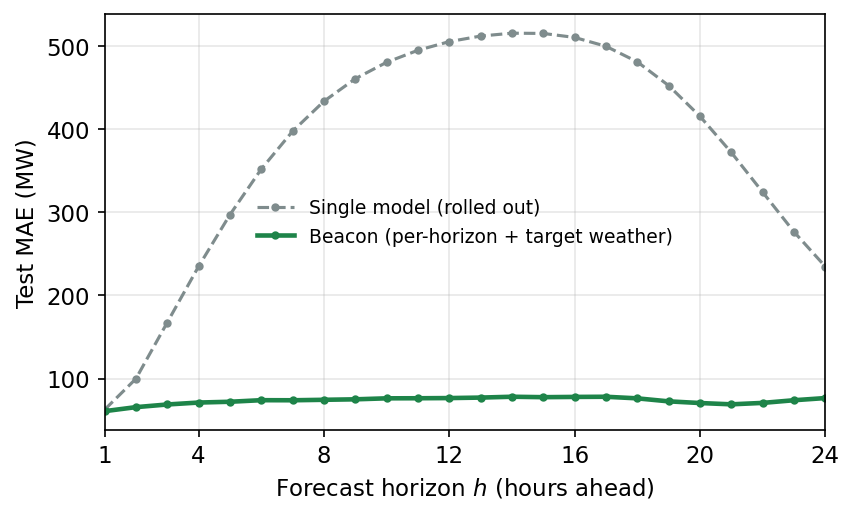
\includegraphics[width=\columnwidth]{fig_horizon_mae.png}
\caption{Per-horizon test-set MAE: Beacon (direct multi-horizon) versus the
single-model rolled-out baseline. Beacon remains flat ($60.9$--$76.7$\,MW),
while the single model collapses at mid-horizons, peaking near $505$\,MW around
$h=12$ where the one-step anchor is least informative.}
\label{fig:horizon}
\end{figure}

\subsection{Live comparison against ISO-NE}
Table~\ref{tab:iso} reports the horizon-matched live evaluation over the
$\sim$30-day, $720$-point window, with both forecasters at the same $24$-hour-ahead
horizon, the same Open-Meteo weather, and ISO-NE real-time demand as ground truth.
Beacon attains an MAE of $89.3$\,MW and a MAPE of $3.50\%$, against ISO-NE's
$92.6$\,MW and $3.70\%$. Beacon thus beats the operational forecast on both MAE
($-3.3$\,MW, $\approx +3.5\%$) and MAPE, while ISO-NE retains a marginally higher
$R^2$ ($0.923$ vs.\ $0.904$). The headline takeaway is that a fully reproducible,
keyless pipeline edges out a mature operational benchmark on absolute error once
the comparison is made honestly horizon-matched. We emphasise that the live window
is short and falls in spring/early-summer, so this result is a like-for-like
demonstration rather than a claim of dominance across all seasons.

\begin{table}[t]
\centering
\caption{Live, horizon-matched day-ahead comparison ($\sim$30-day window,
$720$ points). Both forecasters at $24$\,h ahead, same Open-Meteo weather,
ISO-NE real-time demand as actuals.}
\label{tab:iso}
\begin{tabular}{lccc}
\toprule
Forecaster & MAE (MW) & MAPE (\%) & $R^2$ \\
\midrule
Beacon (day-ahead) & $\mathbf{89.3}$ & $\mathbf{3.50}$ & $0.904$ \\
ISO-NE (day-ahead)  & $92.6$ & $3.70$ & $\mathbf{0.923}$ \\
\bottomrule
\end{tabular}
\end{table}

\subsection{Ablations}
Table~\ref{tab:ablation} decomposes the day-ahead gains into two cumulative
changes, with Figure~\ref{fig:ablation} visualising the day-ahead ($h=24$) MAE
across the three configurations. Starting from a lags-only model served
OpenWeatherMap (OWM) weather, the day-ahead MAE is $183.0$\,MW (with $h=1$ at
$78.7$\,MW). Adding the target-hour exogenous features---the forecasted weather
and exactly-known calendar at hour $t+h$---cuts the day-ahead MAE to $110.3$\,MW
(a $\approx 40\%$ reduction) while leaving $h=1$ essentially unchanged at
$77.7$\,MW, as expected since the nowcast already has its target-hour context.
Finally, unifying the weather source on Open-Meteo for both training and serving
drops the day-ahead MAE to $76.7$\,MW and, notably, improves $h=1$ to $60.9$\,MW.

\begin{table}[t]
\centering
\caption{Cumulative ablation of target-hour features and weather source
(test-set MAE, MW).}
\label{tab:ablation}
\begin{tabular}{lcc}
\toprule
Configuration & MAE @ $h=1$ & MAE @ $h=24$ \\
\midrule
Lags only, OWM weather & $78.7$ & $183.0$ \\
\;+ target-hour features, OWM & $77.7$ & $110.3$ \\
\;+ Open-Meteo (matched) --- \textbf{final} & $\mathbf{60.9}$ & $\mathbf{76.7}$ \\
\bottomrule
\end{tabular}
\end{table}

\begin{figure}[t]
\centering
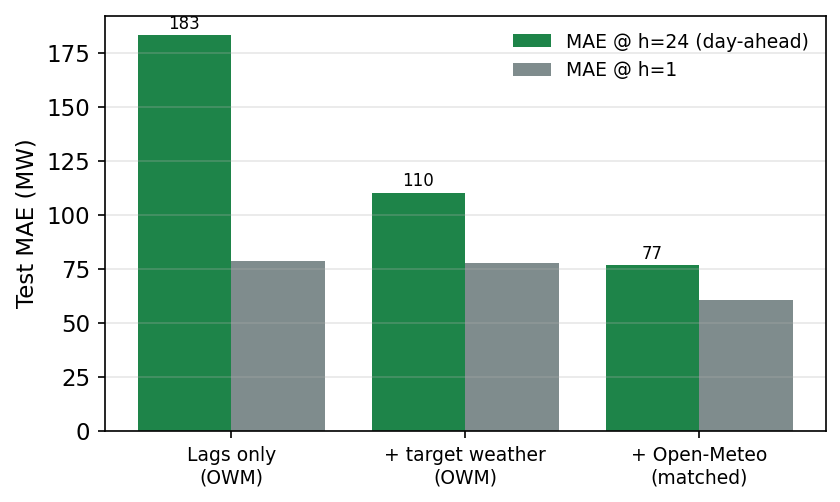
\includegraphics[width=\columnwidth]{fig_ablation.png}
\caption{Day-ahead ($h=24$) test-set MAE across the three cumulative
configurations: lags-only ($183.0$\,MW) $\rightarrow$ $+$ target-hour weather
($110.3$\,MW) $\rightarrow$ $+$ Open-Meteo train/serve matching ($76.7$\,MW).}
\label{fig:ablation}
\end{figure}

The deployment consequence of the weather source is sharper still. A model trained
on OpenWeatherMap CSVs but served Open-Meteo weather suffers a live day-ahead MAE
of $\approx 147$\,MW; retraining on Open-Meteo to match the serving source brings
this down to $\approx 90$\,MW---essentially the ISO-NE level ($\approx 92$\,MW).
Matching the train/serve weather source alone thus removes most of the gap to the
operational benchmark, underscoring that a silent train/serve distribution
mismatch can nearly double deployed error.

\subsection{Leakage audit}
Finally, Table~\ref{tab:leak} reports the shuffled-target test, the gold standard
for detecting feature--target leakage. With genuine targets the test $R^2$ is
$0.956$ at $h=1$ and $0.770$ at $h=24$; when the targets are randomly permuted
before training, $R^2$ collapses to $-0.019$ and $-0.021$ respectively---no better
than predicting the mean. This confirms the model exploits real feature--target
structure rather than any inadvertent leakage. The monotone increase of MAE with
horizon documented in Figure~\ref{fig:horizon} is corroborating evidence: a leaking
model would remain near-flat across horizons rather than degrade in the orderly,
physically plausible way Beacon does.

\begin{table}[t]
\centering
\caption{Leakage audit: real-target versus shuffled-target test $R^2$.}
\label{tab:leak}
\begin{tabular}{lcc}
\toprule
Horizon & Real-target $R^2$ & Shuffled-target $R^2$ \\
\midrule
$h=1$  & $0.956$ & $-0.019$ \\
$h=24$ & $0.770$ & $-0.021$ \\
\bottomrule
\end{tabular}
\end{table}

\section{Discussion}\label{sec:discussion}

\subsection{Target-hour weather is the day-ahead lever}
The results in Section~\ref{sec:results} make clear that the dominant lever for
day-ahead accuracy is not the recent load history but the \emph{forecasted weather
at the target hour}. Twenty-four hours out, the most recent observed load carries
comparatively little information about tomorrow's load: the diurnal and weather-driven
structure of the day to come is what matters, and that structure is captured by
calendar features (exactly known in advance) and by the forecast temperature at
$t+h$. Because each per-horizon model is trained to read the exogenous features at its
own target hour rather than rolling a near-term prediction forward, it stays accurate
deep into the horizon. The ablation in Table~\ref{tab:ablation} quantifies this:
adding target-hour calendar and weather features cuts day-ahead (h=24) MAE from
$183.0$ to $110.3$~MW, and unifying the weather source pushes it further to
$76.7$~MW. The bulk of the day-ahead error that a lags-only model exhibits is, in
effect, an absence of knowledge about tomorrow's weather, not an absence of recent
load.

\subsection{Train/serve weather-source matching}
A second, more subtle lesson concerns deployment. A model can be internally
consistent and well-validated on held-out data yet still degrade in production if the
distribution of an input shifts silently between training and serving. Here the
culprit was the weather source: training on OpenWeatherMap history while serving
Open-Meteo forecasts induced a distribution mismatch that nearly doubled live
day-ahead error, from roughly $90$ to $147$~MW (Section~\ref{sec:results}). Retraining
on the same Open-Meteo source used at serving time removed most of the gap to the
operator. No change to the model architecture, features, or hyper-parameters was
involved; the single act of \emph{matching the train and serve weather source} was
responsible. For weather-informed forecasters this is an easy mistake to make and a
costly one, and it argues for treating the exogenous-data provider as a versioned,
unified part of the pipeline rather than an interchangeable commodity.

\subsection{The horizon-mismatch pitfall}
The comparison against ISO-NE also illustrates a methodological pitfall that can
inflate reported gains. It is tempting to compare a model's short-horizon nowcast
against an operator's day-ahead forecast, but this is not an apples-to-apples
contrast: the two forecasts solve different problems at different lead times. When the
comparison is made honestly --- both forecasters evaluated at the same 24-hour-ahead
horizon, on the same Open-Meteo weather --- Beacon's edge over the ISO-NE operational
forecast is a modest but real improvement of $-3.3$~MW MAE ($\approx +3.5\%$), with a
corresponding MAPE improvement and a marginally lower $R^2$ (Table~\ref{tab:iso}).
This is a genuine result, not the inflated figure a horizon mismatch would produce,
and reporting it as such is part of the contribution.

\subsection{Operational implications}
Taken together, these findings carry a practical message. ISO-NE's day-ahead demand
forecast is an operational product that grid operators rely on for unit commitment,
economic dispatch, and reserve sizing, and matching --- let alone slightly beating ---
it is a hard bar. That a keyless, fully reproducible pipeline built entirely on free
public data sources (ISO-NE Web Services and Open-Meteo) can clear that bar at
day-ahead horizon, while remaining auditable and leakage-clean
(Section~\ref{sec:results}), suggests that the gains here come from disciplined feature
construction and honest evaluation rather than from proprietary data or heavy modeling
machinery. Small MAE reductions translate into meaningful cost and reliability gains in
wholesale electricity markets, and a transparent pipeline that achieves them lowers the
barrier to adoption and independent verification.

\section{Limitations and Future Work}\label{sec:limits}

Several limitations bound the scope of these results. First, the study covers a
\emph{single} reliability zone, NEMA (Northeast Massachusetts / Boston); whether the
same feature design and source-matching discipline transfer to other ISO-NE zones, or
to other markets with different load shapes and weather regimes, remains to be shown.
Second, the live horizon-matched evaluation against ISO-NE spans only about $30$ days
of spring and early summer. This window is short and seasonally narrow: it excludes
peak-summer cooling load and winter heating extremes, the periods where day-ahead
forecasting is most consequential and most difficult. The test-set results
(Section~\ref{sec:results}) draw on a full year of held-out 2025 data and are
correspondingly more robust, but the head-to-head with the operator should be read as
indicative rather than conclusive.

Third, the load series differ slightly between the training source (wholesale-load,
WHLSECOST) and the real-time-demand series used as live actuals; small definitional
differences between these series add noise to the live comparison. Fourth, the
Open-Meteo ERA5 archive does not provide a visibility channel, which was filled with a
constant during training; visibility is therefore inert as a feature. Finally, Beacon
produces \emph{point} forecasts only --- it emits no predictive intervals or quantile
bands, which limits its usefulness for reserve sizing and risk-aware dispatch, where
uncertainty quantification is valuable.

These limitations map onto a clear program of future work. The most immediate
extension is \emph{probabilistic} forecasting: quantile or interval bands around each
per-horizon prediction, so that the forecaster communicates uncertainty rather than a
single number. Beyond point accuracy, ensembling the gradient-boosted models with a
transformer-style sequence model such as Informer~\cite{zhou2021informer} may capture
longer-range temporal structure that the lag features miss. Broader evaluation ---
extending across all ISO-NE zones and across a full seasonal cycle --- would test
generalization directly. Systematic hyper-parameter search via Optuna, and
recency-weighted retraining that adapts to gradual changes in load behavior, are
natural refinements to the training procedure that we leave to future work.

\section{Conclusion}\label{sec:conclusion}

This paper presented Beacon, a direct multi-horizon gradient-boosting forecaster for
day-ahead hourly load in the NEMA zone of ISO New England. Rather than rolling a
single near-term model forward, Beacon trains $24$ independent CatBoost models, one per
horizon, each reading a $168$-hour lookback window together with the calendar and
\emph{forecasted weather at its own target hour}. This design removes recursive error
compounding and makes tomorrow's forecasted temperature --- the dominant driver of
day-ahead load --- directly available to every horizon model.

The contributions are fourfold: a direct per-horizon design that lowers average MAE by
$80.6\%$ relative to a single-model roll-out; target-hour exogenous features as the
lever that cuts day-ahead MAE from $183$ to $77$~MW; identification and correction of a
train/serve weather-source mismatch that had nearly doubled live error; and a
horizon-matched, leakage-audited evaluation protocol against an operational ISO
forecast. On a full year of held-out 2025 data, Beacon attains a day-ahead (h=24) MAE
of $76.7$~MW. In a live, horizon-matched comparison over a $30$-day window, it reaches
a day-ahead MAE of $89.3$~MW against ISO-NE's $92.6$~MW, slightly beating the
operational forecast on MAE and MAPE while remaining marginally behind on $R^2$. A
shuffled-target test confirms the models exploit genuine feature--target structure
rather than leakage.

That a keyless, fully reproducible pipeline built on free public data can match and
modestly beat a professional operational forecast --- once the comparison is made
honestly --- suggests that careful feature construction, source discipline, and honest
evaluation matter as much as model complexity. We hope the methodological lessons,
particularly the two pitfalls this work highlights, prove useful to practitioners
deploying weather-informed load forecasters.


\section*{Reproducibility}
All code, trained models, and metric artefacts are available at
\href{https://github.com/arunnath011/NEMA}{github.com/arunnath011/NEMA}. Weather is sourced from
the keyless Open-Meteo API; live load and the day-ahead benchmark from the ISO New England Web
Services API.

\bibliographystyle{plain}
\bibliography{references}

\end{document}
